%%%%%%%%%%%%%%%%%%%%%%%%%%%%%%%%%%%%%%%%%%%%%%%%%%%%%%%%%%
%%
%% MARK: Title
%%
%%%%%%%%%%%%%%%%%%%%%%%%%%%%%%%%%%%%%%%%%%%%%%%%%%%%%%%%%%

\chapter*{\S B5. Infinite Torus Action on Smooth Periodic Functions}
\setcounter{footnote}{0}

%%%%%%%%%%%%%%%%%%%%%%%%%%%%%%%%%%%%%%%%%%%%%%%%%%%%%%%%%%
%%
%% MARK: Abstract
%%
%%%%%%%%%%%%%%%%%%%%%%%%%%%%%%%%%%%%%%%%%%%%%%%%%%%%%%%%%%

\begin{abstract}
  We continue the previous exercise on the space of Fourier coefficients
  of smooth periodic functions, equipped with the functional diffeology,
  by considering the infinite product $\Torus^\infty$ of tori $\U(1)$
  as a group of diffeomorphisms.
\end{abstract}

%%%%%%%%%%%%%%%%%%%%%%%%%%%%%%%%%%%%%%%%%%%%%%%%%%%%%%%%%%
%%
%% MARK: Introduction
%%
%%%%%%%%%%%%%%%%%%%%%%%%%%%%%%%%%%%%%%%%%%%%%%%%%%%%%%%%%%

We denote by $\Torus^\infty$ the set of infinite sequences $\tau = (\tau_n)_{n\in \ZZ}$, where $\tau_n \in  \Torus = \U(1)$,
that is,
$\tau_n \in \CC$ and $\bar \tau_n \tau_n = 1$:
$$
  \Torus^\infty = \prod_{n \in \ZZ} \U(1).
  $$
Let $\cE$ be the set of Fourier coefficients of smooth $1$-periodic functions equipped with the pushforward of the
functional diffeology, as it is described in ``Functional Diffeology on Fourier Coefficients''.
There is a natural linear action of $\Torus^\infty$ on $\cE$,
defined by
$$
  \tau \cdot Z = (\tau_n)_{n \in \ZZ} \cdot (Z_n)_{n \in \ZZ} = (\tau_n Z_n)_{n \in \ZZ}.
  $$
Indeed, multiplying by a number of modulus 1 transforms a rapidly decreasing sequence of complex numbers into another,
and every $\tau=(\tau_n)_{n \in \ZZ} \in \Torus^\infty$ is invertible
$$
  (\tau_n)_{n \in \ZZ}^{-1} = (\bar \tau_n)_{n \in \ZZ}.
  $$
Moreover, for every plot $r \mapsto (Z_n(r))_{n\in \ZZ}$ in $\cE$, for all $p \in \NN$,
$$
  \left|{\partial^p \tau_n Z_n(r) \over \partial r^p}\right| % = \left|z_n {\partial^p Z_n(r) \over \partial r^p}\right|
  = \left|{\partial^p Z_n(r) \over \partial r^p}\right|.
  $$
The same holds for the inverse. Hence, the action of $(\tau_n)_{n \in \ZZ}$ is smooth as well as its inverse, thus $(\tau_n)_{n \in \ZZ}$
acts by diffeomorphism. We have then a monomorphism
$$
  \eta : \Torus^\infty \to \GL^\infty(\cE).
  $$

%%%%%%%%%%%%%%%%%%%%%%%%%%%%%%%%%%%%%%%%%%%%%%%%%%%%%%%%%%
%%
%% MARK: Exercise 1
%%
%%%%%%%%%%%%%%%%%%%%%%%%%%%%%%%%%%%%%%%%%%%%%%%%%%%%%%%%%%

\begin{Article}{Exercise I.}{}
  We consider the group $\Torus^\infty$ of diffeomorphisms of $\cE$.
  We shall say that a parametrization $r \mapsto \tau(r) = (\tau_n(r))_{n\in \ZZ}$ in $\Torus^\infty$ is {\em tempered} if the $\tau_n$ are smooth and if for every $k \in \NN$,
  for every $r_0$ in the domain of the parametrization,
  there exists a ball $\cB$ centered at $r_0$,
  a polynomial $P_k(n)$,
  and an integer $N$ such that
  \begin{equation}
    \renewcommand{\theequation}{$\spadesuit$}
    \forall r \in \cB, \forall n > N, \quad \left|{\partial^k \tau_n(r) \over \partial r^k}\right| \leq P_k(n).
  \end{equation}
  
  \Question {Q1.} Show that the tempered parametrizations form a group diffeology on $\Torus^\infty$.
  
  \Question {Q2.} Show that, equipped with the tempered diffeology, the action of the group $\Torus^\infty$
  on $\cE$ is smooth.
  
  \Question {Q3.} Show that for all $N \in \NN$, the injection $\iota_N : \Torus^N \to \Torus^\infty$ defined
  by
  $$
    \iota_N(\zeta) = \tau \SpacedText{with}  \left\{
    \begin{array}{ll}
    \tau_n = \zeta_n & \mbox{if $n \in \{1,\ldots,N\}$}, \\
    \tau_n = 1  & \mbox{otherwise},
    \end{array}
    \right.
    $$
  is an induction.
\end{Article}

\begin{proof}
  For Question 1. Let us show that the condition $(\spadesuit)$ defines a diffeology, actually a sub-diffeology of the
  product diffeology on the infinite product of tori $\Torus^\infty = \prod_{n\in \ZZ} \Torus$.
  We denote indifferently $\U(1)$ or $\Torus$,
  for Torus.
  
  {(Covering axiom)} If $\tau_n(r) = \tau_n$ is constant in $r$, for all $n$,
  then $\Modulus{\partial^k \tau_n(r)/\partial r^k}$ is equal to $1$ for $k = 0$ and equal to $0$ for $k>0$.
  It satisfies the condition $(\spadesuit)$.
  
  {(Locality axiom)} By definition the condition $(\spadesuit)$ is local in the variable $r$.
  
  {(Smooth compatibility axiom)} Let $\tau : r \mapsto \tau_n(r)_{n\in \ZZ}$
  satisfying $(\spadesuit)$ and $F : s \mapsto r$
  be a smooth parametrization in the domain of $\tau$.
  We have, for all $k>0$,
  $$
    {\partial^k \tau_n(s) \over \partial s^k} = \sum_{\ell = 1}^{k}
    {\partial^\ell \tau_n(r) \over \partial r^\ell} \cdot
    Q_{k,\ell}\left({\partial r \over \partial s},\ldots,{\partial^k r \over \partial s^k}\right),
    $$
  where the $Q_{k,\ell}$ are polynomials. Therefore,
  $$
    \left|{\partial^k \tau_n(s) \over \partial s^k}\right| \leq \sum_{\ell = 1}^{k}
    \left|{\partial^\ell \tau_n(r) \over \partial r^\ell}\right| \,
    \left| \vphantom{{\partial^\ell \tau_n(r) \over \partial r^\ell}} Q_{k,\ell}\left({\partial r \over \partial s},\ldots,{\partial^k r \over \partial s^k}\right)\right|.
    $$
  Since the function $s\mapsto r$ is smooth, these polynomials are locally absolutely bounded, let
  $$
    M_{k,\ell} = \Sup_{r \in \cB}
    \left|Q_{k,\ell}\left({\partial r \over \partial s},\ldots,{\partial^k r \over \partial s^k}\right)\right|.
    $$
  Next, let $N_\ell$ satisfying ($\spadesuit$) for $k=\ell$, and $N' = \Sup_{\ell = 1\ldots k} N_\ell$, then
  for all $n>N'$,
  $$
    \left|{\partial^k \tau_n(s) \over \partial s^k}\right| \leq \sum_{\ell = 1}^{k}
    M_{k,\ell}\left|{\partial^\ell \tau_n(r) \over \partial r^\ell}\right| \leq \sum_{\ell = 1}^{k}
    M_{k,\ell}P_\ell(n).
    $$
  Hence, the partial derivatives of the $\tau_n$ with respect to $r$ are still dominated by polynomials, and
  the condition $(\spadesuit)$ defines a diffeology on the set $\Torus^\infty$.
  
  For Question 2. Now, let us check that $(\spadesuit)$ defines
  a group diffeology. First of all, let $\tau : r \mapsto (\tau_n(r))_{n\in\ZZ}$ and
  $\tau' : r \mapsto (\tau'_n(r))_{n\in\ZZ}$ be two plots of $\Torus^\infty$, the derivatives of the
  terms of the product $\tau_n(r)\tau'_n(r)$ write
  $$
    {\partial^k \tau_n(r)\tau'_n(r) \over \partial r^k} = \sum_{\ell = 1}^{k}
    {k \choose \ell}
    {\partial^{k-\ell} \tau_n(r) \over \partial r^{k-\ell}} \cdot
    {\partial^{\ell} \tau'_n(r) \over \partial r^{\ell}}.
    $$
  Hence,
  \begin{eqnarray*}
    \left|{\partial^k \tau_n(r)\tau'_n(r) \over \partial r^k} \right|
    & \leq & \sum_{\ell = 1}^{k} {k \choose \ell} \left|{\partial^{k-\ell} \tau_n(r) \over \partial r^{k-\ell}}\right| \,
    \left|{\partial^{\ell} \tau'_n(r) \over \partial r^{\ell}}\right| \\
    & \leq & \sum_{\ell = 1}^{k} {k \choose \ell} P_{k-\ell}(n) \, P'_\ell(n).
  \end{eqnarray*}
  The partial derivatives of the product $\tau_n \tau'_n$ are still dominated by a polynomial.
  The inverse mapping is given by $\iota : (\tau_n)_{n\in\ZZ} \mapsto (\bar \tau_n)_{n\in\ZZ}$,
  the absolute values of the partial derivatives of each component and its inverse coincide.
  Therefore,
  $\Torus^\infty$, equipped with the diffeology
  $(\spadesuit)$ is a diffeological group.
  
  For Question 3. The injection $\iota_N : \Torus^N \to \Torus^\infty$ is clearly smooth since,
  for all plots $\tau$ in $\Torus^N$,
  the derivatives of the components $\tau_n$ of the composite $\iota_N \circ \tau : r \mapsto (\tau_n(r))_{n\in\ZZ}$ vanish for $n$ outside $\{1,\ldots,N\}$,
  hence
  $$
    n^p\,{\partial^k \tau_n(r) \over \partial r^k} = 0 \SpacedText{if $\Modulus{n} > N$.}
    $$
  Conversely if $\tau : r \mapsto (\tau_n(r))_{n\in\ZZ}$ is a plot in $\Torus^\infty$ with values in $\iota_N(\Torus^N)$,
  then the components $r \mapsto \tau_n(r)$ are smooth,
  by definition of the diffeology on $\Torus^\infty$,
  and hence $\iota_N^{-1}\circ \tau$ is smooth.
  Therefore,
  $\iota_N$ is an induction.
\end{proof}

%%%%%%%%%%%%%%%%%%%%%%%%%%%%%%%%%%%%%%%%%%%%%%%%%%%%%%%%%%
%%
%% MARK: Exercise 2
%%
%%%%%%%%%%%%%%%%%%%%%%%%%%%%%%%%%%%%%%%%%%%%%%%%%%%%%%%%%%

\begin{Article}{Exercise II.}{}
  Let $\alpha = (\alpha_n)_{n\in\ZZ}$ be a sequence of positive irrational numbers independent over $\QQ$, that is,
  for every sequence $(q_n)_{n\in\ZZ}$, with finite support, of rational numbers $q_n \in \QQ$ one has
  $$
    \sum_{n\in\ZZ} q_n \alpha_n = 0 \quad \Rightarrow \quad q_n = 0 \SpacedText{for all} n.
    $$
  \Question{Q1.} Give an example of such a family of irrational numbers.
  
  \Question{Q2.} Show that $\iota : \RR \mapsto \Torus^\infty$, defined by
  $$
    \iota(t) = \bigg(e^{2i\pi\alpha_n t}\bigg)_{n\in \ZZ},
    $$
  is an induction.
\end{Article}

\begin{proof}
  For Question 1. Consider a transcendent number $\alpha$ (we assume $\alpha<1$ even if it is not necessary). We define
  $$
    \alpha_0 = 1 \SpacedText{and} \alpha_m = \alpha^m - \left[{\alpha^m}\right] \quad \mbox{for $m\neq0$},
    $$
  where the bracket denotes the integral part.
  That defines $\alpha_n$ for all $n\in \ZZ$.
  Now,
  for a finitely supported sequence of rational numbers $q_n$, we have
  \begin{eqnarray*}
    \sum_{n\in \ZZ} q_n \alpha_n & = & q_0 + \sum_{n \in \ZZ \atop n\neq 0}
    q_n\left(\alpha^n -
    [\alpha^n]\right) \\
    &=& q_0 - \sum_{n \in \ZZ \atop n\neq 0} q_n [\alpha^n] + \sum_{n \in \ZZ \atop n\neq 0} q_n\alpha^n,
  \end{eqnarray*}
  with only finitely many terms non-zero.
  Then,
  if $\sum_{n\in\ZZ} q_n \alpha_n =0$ we multiply
  both sides by $\alpha^\ell$,
  with $\ell$ big enough to get an algebraic equation in $\alpha$,
  with all powers positive.
  But we assumed $\alpha$ transcendent,
  then all the coefficients are $0$,
  what implies $q_n= 0$,
  for all $n\in \ZZ$.
  
  For Question 2.
  We need to check first of all that $\iota$ is smooth.
  The successive derivatives are simply
  $$
    {\partial^k e^{2i\pi\alpha_n t} \over \partial t^k} = (2i\pi\alpha_n)^k e^{2i\pi\alpha_n t}.
    $$
  Since $0<\alpha_n \leq 1$, for all $n \in \ZZ$, we have
  $$
    \left|{\partial^k e^{2i\pi\alpha_n t} \over \partial t^k}\right| \leq (2\pi)^k.
    $$
  Hence,
  the derivatives are absolutely dominated by (constant) polynomials and $\iota$ is a plot in $\Torus^\infty$.
  Next,
  consider a plot in $\Torus^\infty$
  with values in $\iota(\RR)$,
  the composite with the projection on the first two components gives a plot in $\Torus^2$ with values in the solenoid
  $$
    (\exp(2i\pi t),\exp(2i\pi\alpha t))_{t\in \RR}.
    $$
  But the injection
  $t \mapsto (\exp(2i\pi t),\exp(2i\pi\alpha t))$ is an induction,
  see \cite[Exercise 31]{PIZ13},
  therefore,
  $\iota$ is an induction.
\end{proof}

\vfill
\centerline{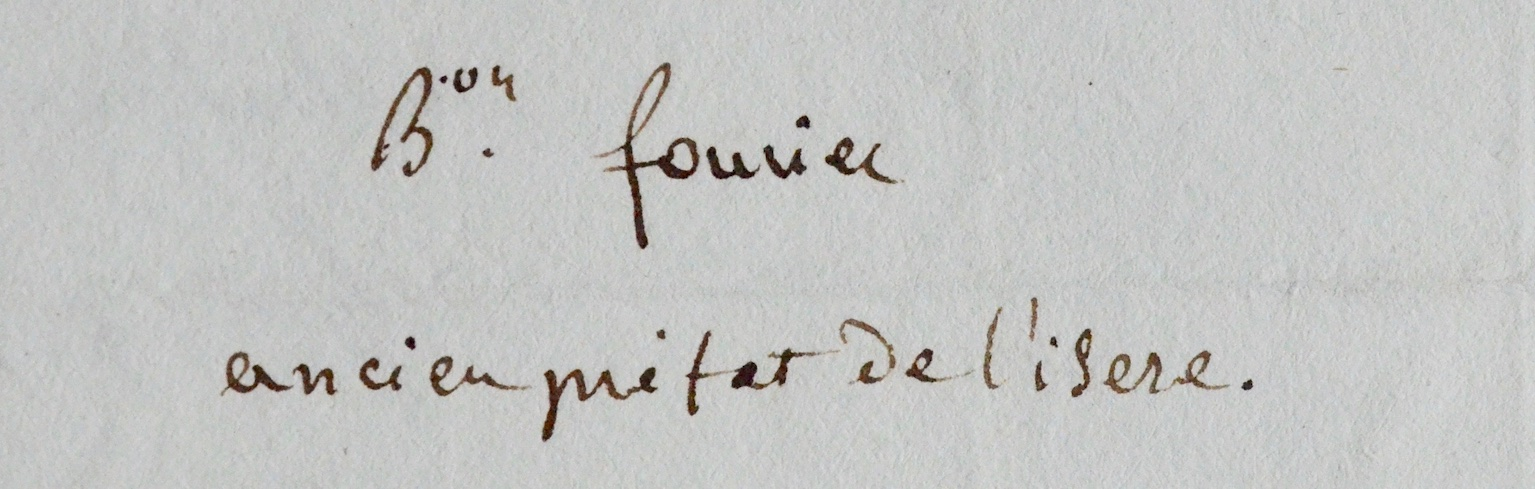
\includegraphics[width=.9\textwidth]{Figures/Fourier-signature.jpg}}
